\documentclass[11pt]{article}
\usepackage{graphicx} % Required for inserting images
\usepackage{amsmath}
\usepackage{fontspec}
\usepackage{polyglossia}
\usepackage{mhchem}
\usepackage{float}
\usepackage{siunitx}
\usepackage[a4paper, top=2cm, bottom=2cm, left=2.5cm, right=2cm]{geometry}
\setmainlanguage{vietnamese}
\setmainfont{Times New Roman}

\title{Báo cáo đo FT-IR của \ce{B-Ag}, \ce{AgO}, \ce{Au-MoS2} trên Base Sillic tại Viện Vật Lý, Viện Hàm Lân Khoa Học và Công Nghệ Việt Nam}
\author{Hoàng Minh Hiếu}
\date{Ngày 6, Tháng 11, 2026}
\begin{document}
\maketitle

\begin{center}
    \textit{Các Base Sillic đều được trải qua quy trình cắt, rửa bằng Acetone, Methanol, DI water và rung siêu âm mỗi chất 15 phút và hotplate làm khô tương tự nhau} 
\end{center}

\section{B-Ag}
- Base vật liệu: Sillic. Vật liệu phủ lên: B-Ag, 1 layer. \newline
- Xử lý bề mặt: Plasma, 2 phút. \newline 
- Spincoat: Nhỏ gián tiếp \newline
\indent{+ Stage 1: 10 giây, 500 rpm.} \newline
\indent{+ Stage 2: 60 giây, 3000 rpm.} \newline
- Ủ nhiệt: Hotplate tại \qty{170}{\degreeCelsius} trong 45 phút.
\begin{figure}[H]
    \centering
    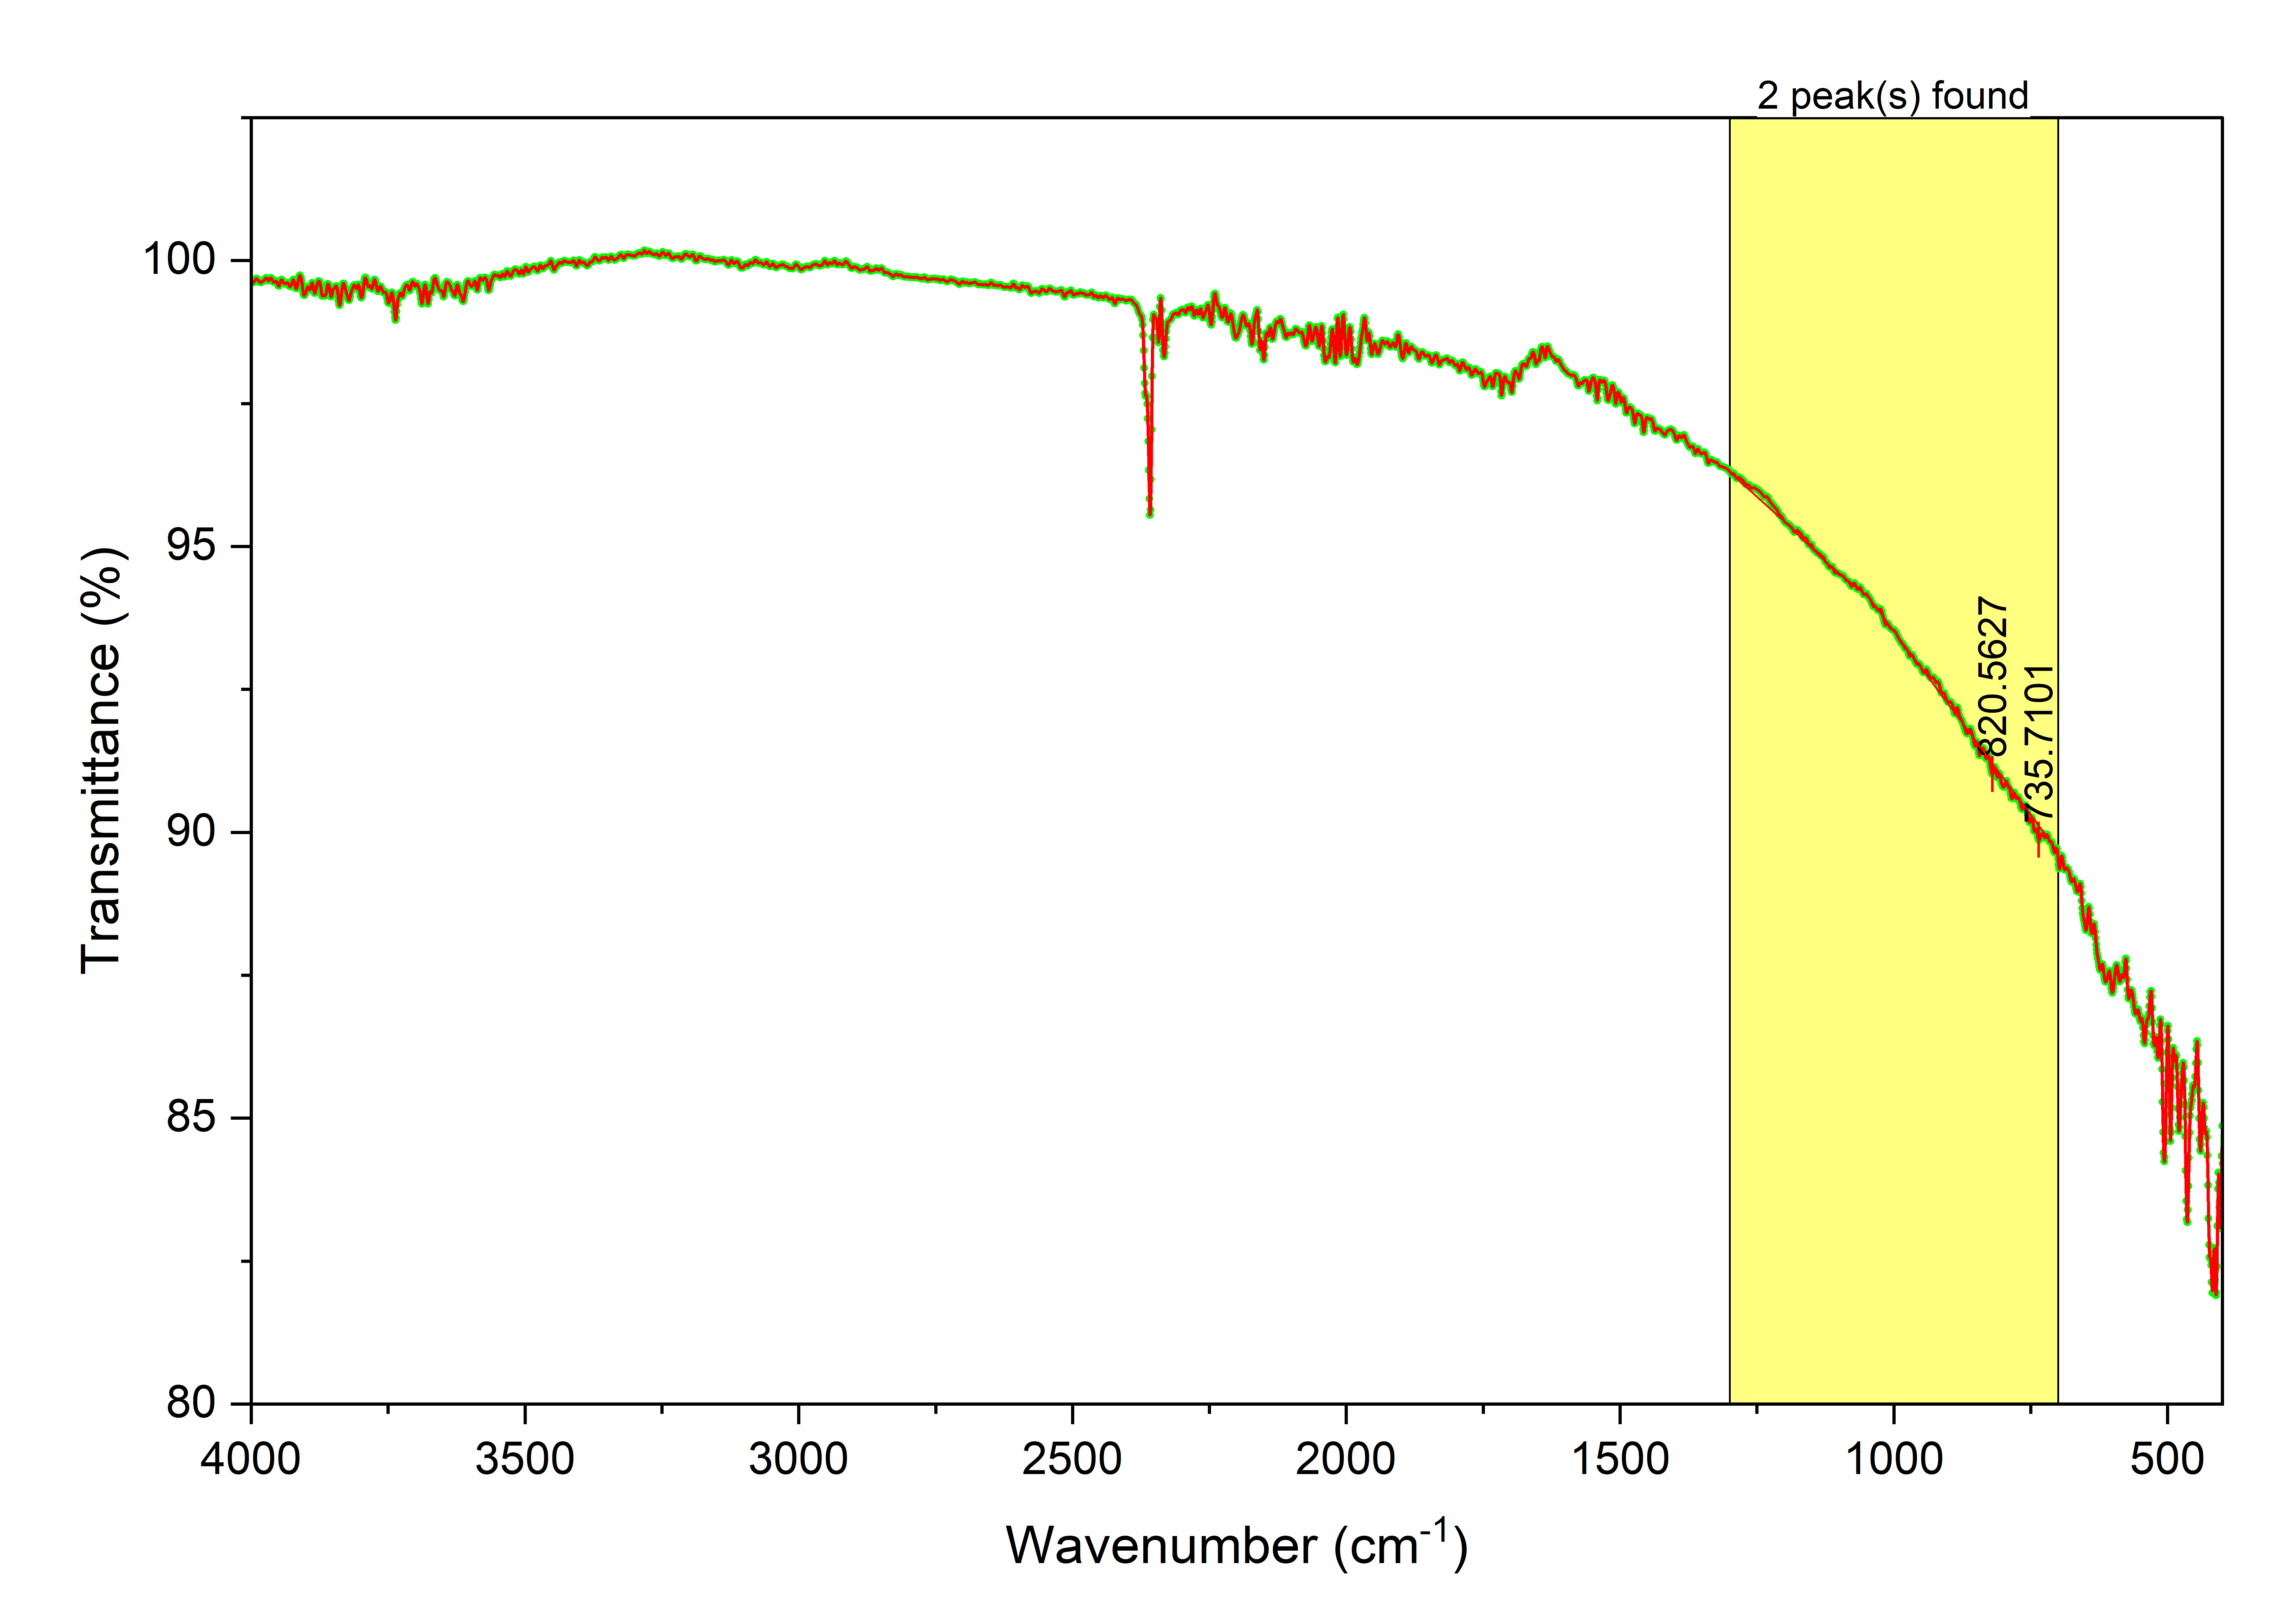
\includegraphics[width=1\textwidth]{B-Ag_SillicBase.png}
    \caption{Phổ FT-IR của mẫu \ce{B-Ag}.}
    \label{fig:ftir_bag}
\end{figure}
2 Peaks: 820$cm^{-1}$, 735$cm^{-1}$. \newline
- Độ truyền qua giảm đều từ ~100\% xuống ~82\% khi đi về số sóng thấp. Đây là nền dốc điển hình do tán xạ hoặc hấp thụ của đế, không phải đặc trưng của lớp phủ. \newline
- Hai đỉnh ở 820 và 735 $cm^{-1}$ rất yếu, chỉ là gợn nhỏ trên nền dốc. Chưa có căn cứ rõ để gán cho liên kết cụ thể.

\section{AgO}
- Base vật liệu: Sillic. Vật liệu phủ lên: \ce{AgO}, 1 layer. \newline
- Xử lý bề mặt: Plasma, 2 phút. \newline 
- Spincoat: Nhỏ gián tiếp \newline
\indent{+ Stage 1: 10 giây, 500 rpm.} \newline
\indent{+ Stage 2: 60 giây, 3000 rpm.} \newline
- Ủ nhiệt: Hotplate tại \qty{170}{\degreeCelsius} trong 45 phút.
\begin{figure}[H]
    \centering
    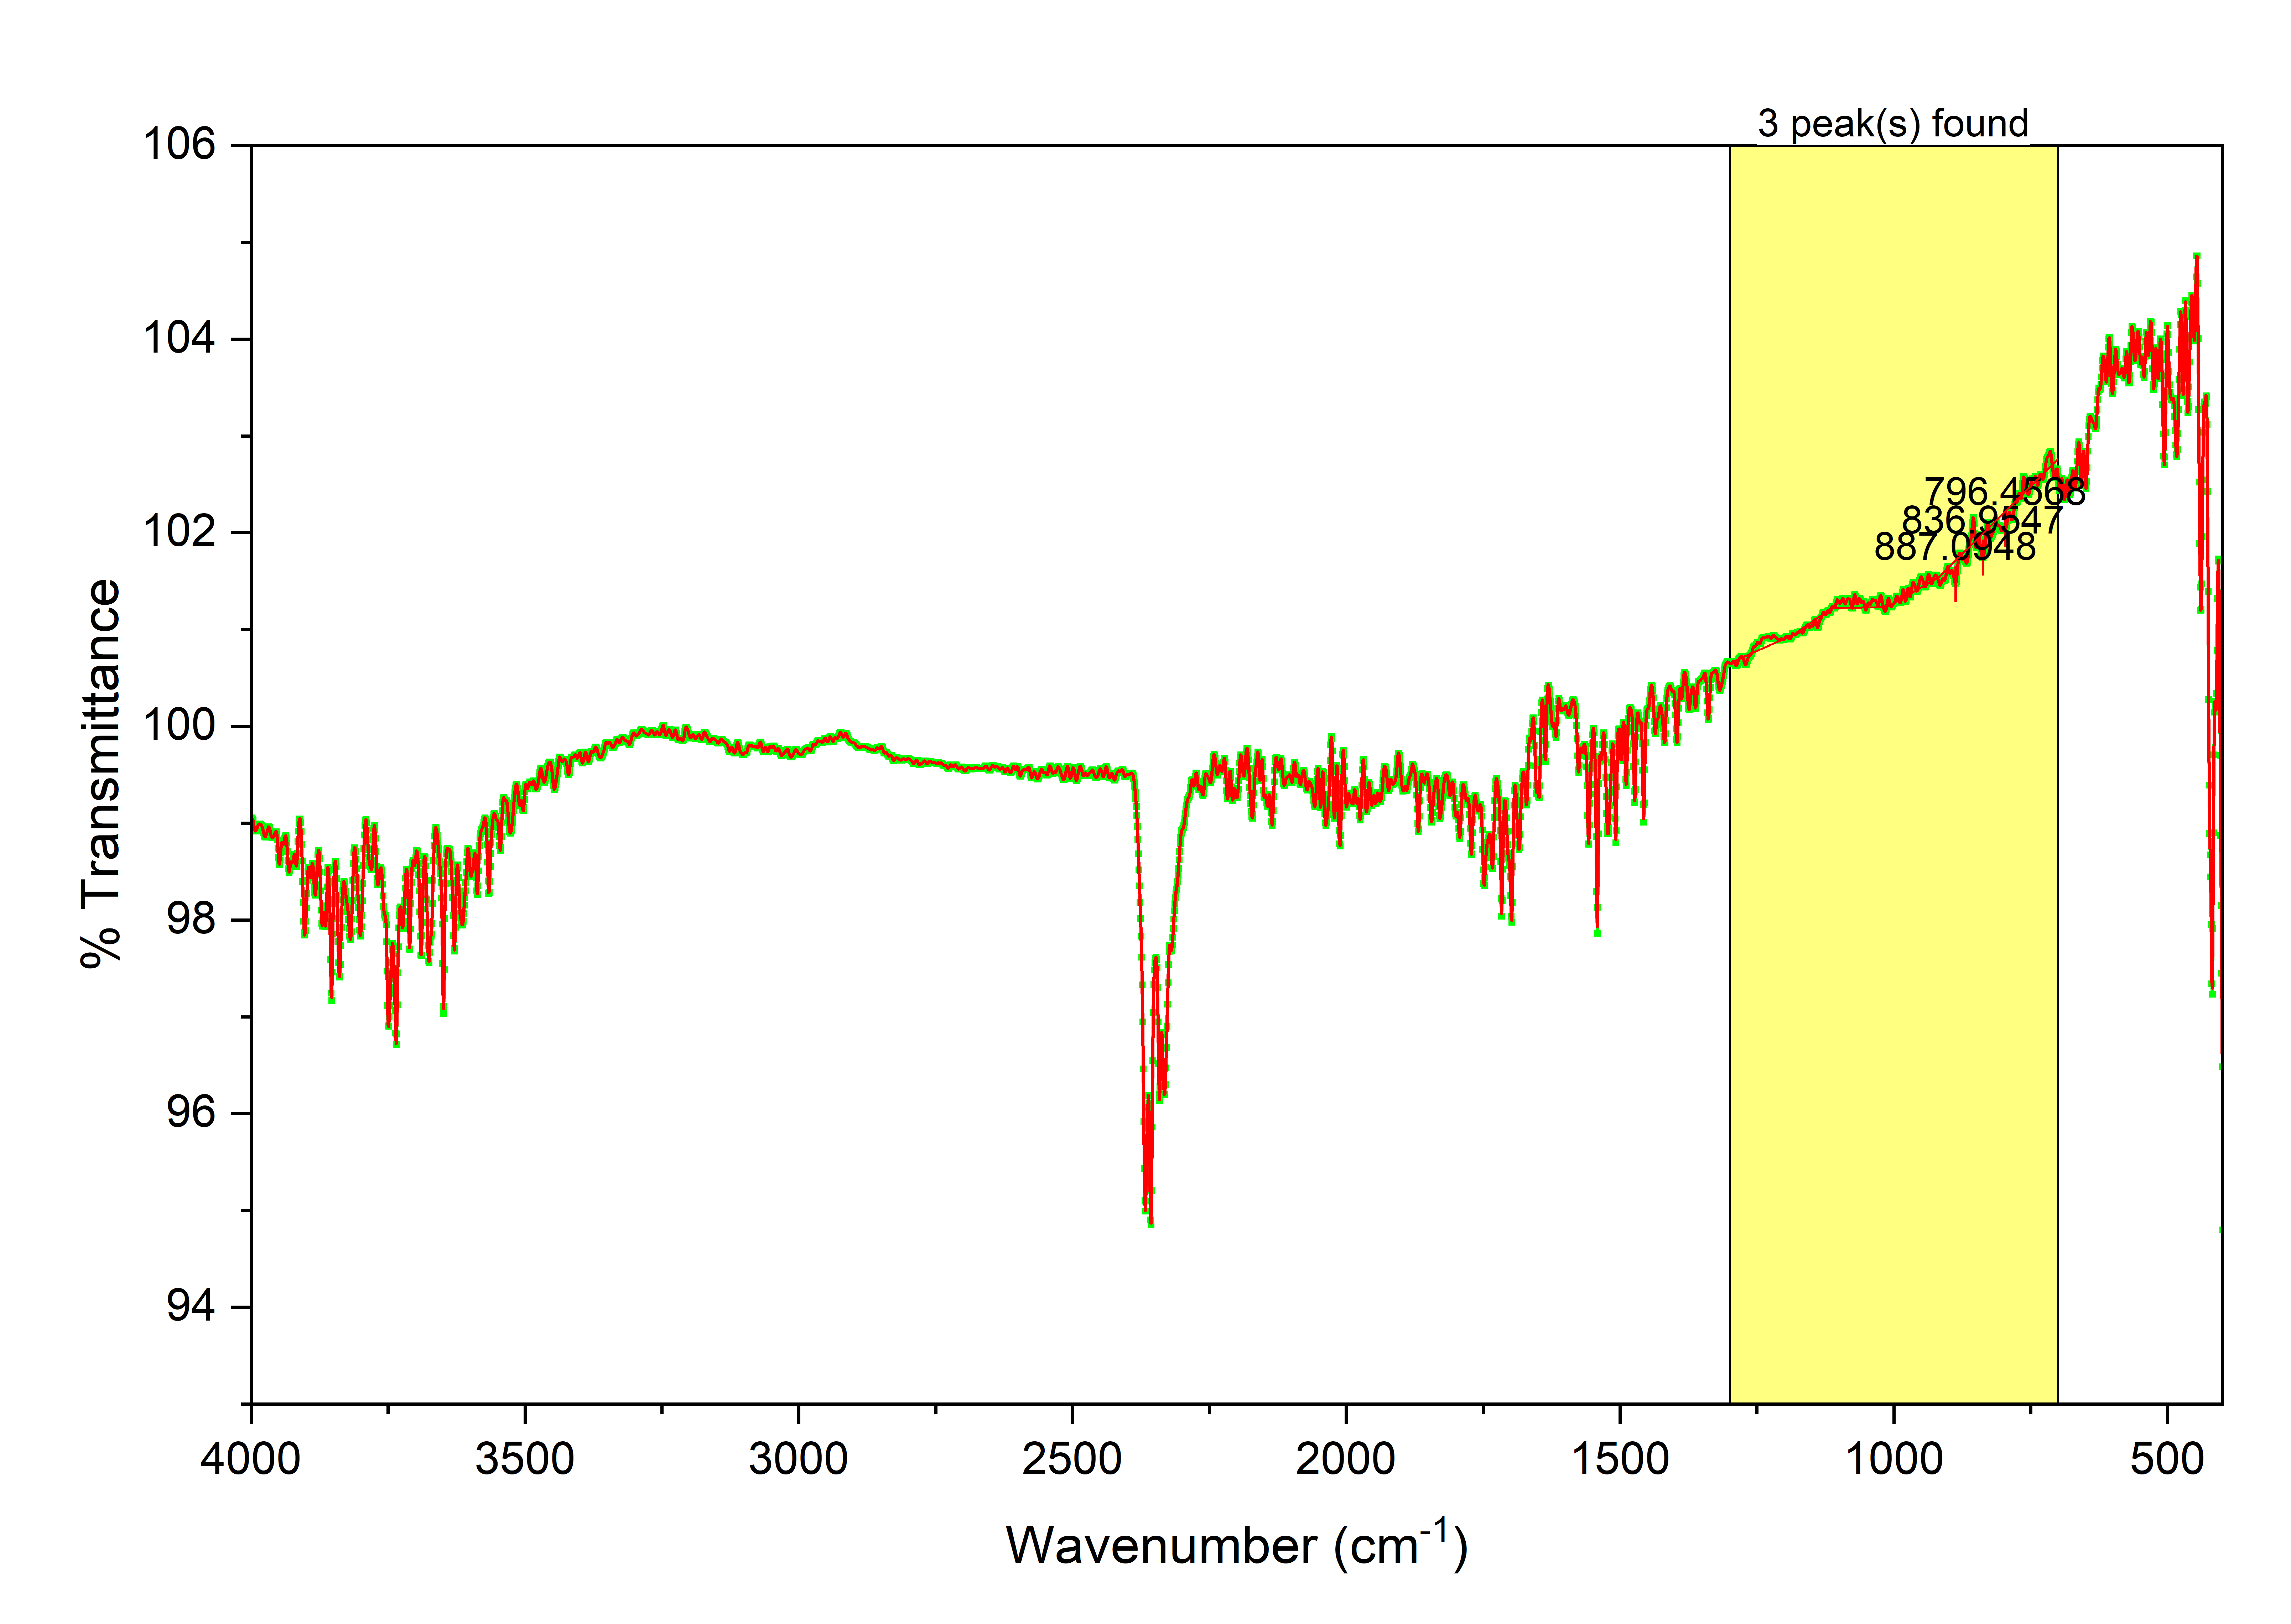
\includegraphics[width=1\textwidth]{AgO_SillicBase.png}
    \caption{Phổ FT-IR của mẫu \ce{AgO}.}
    \label{fig:ftir_ago}
\end{figure}
3 Peaks: 887 $cm^{-1}$, 836 $cm^{-1}$, 796 $cm^{-1}$. \newline
- Nền tăng lên trên 100\% (đến ~104\%). Độ truyền qua > 100\% là phi vật lý, cho thấy phổ nền và phổ mẫu không khớp (ví dụ độ dày hoặc phản xạ của đế khác nhau). Bạn nên ghi rõ điều này trong nhận xét. \newline
- Ba đỉnh chỉ là vai nhỏ trên nền đang dốc lên, các nhãn cũng chồng lên nhau. Liên kết Ag-O thường được báo cáo ở vùng thấp hơn (~400-650 $cm^{-1}$), mà đoạn này lại nhiễu mạnh, nên không kết luận được.

\section{\ce{Au-MoS2}}
- Base vật liệu: Sillic. Vật liệu phủ lên: \ce{Au-MoS2}, 1 layer. \newline
- Xử lý bề mặt: Plasma, 2 phút. \newline 
- Spincoat: Nhỏ gián tiếp \newline
\indent{+ Stage 1: 10 giây, 500 rpm.} \newline
\indent{+ Stage 2: 60 giây, 3000 rpm.} \newline
- Ủ nhiệt: Hotplate tại \qty{170}{\degreeCelsius} trong 45 phút.
\begin{figure}[H]
    \centering
    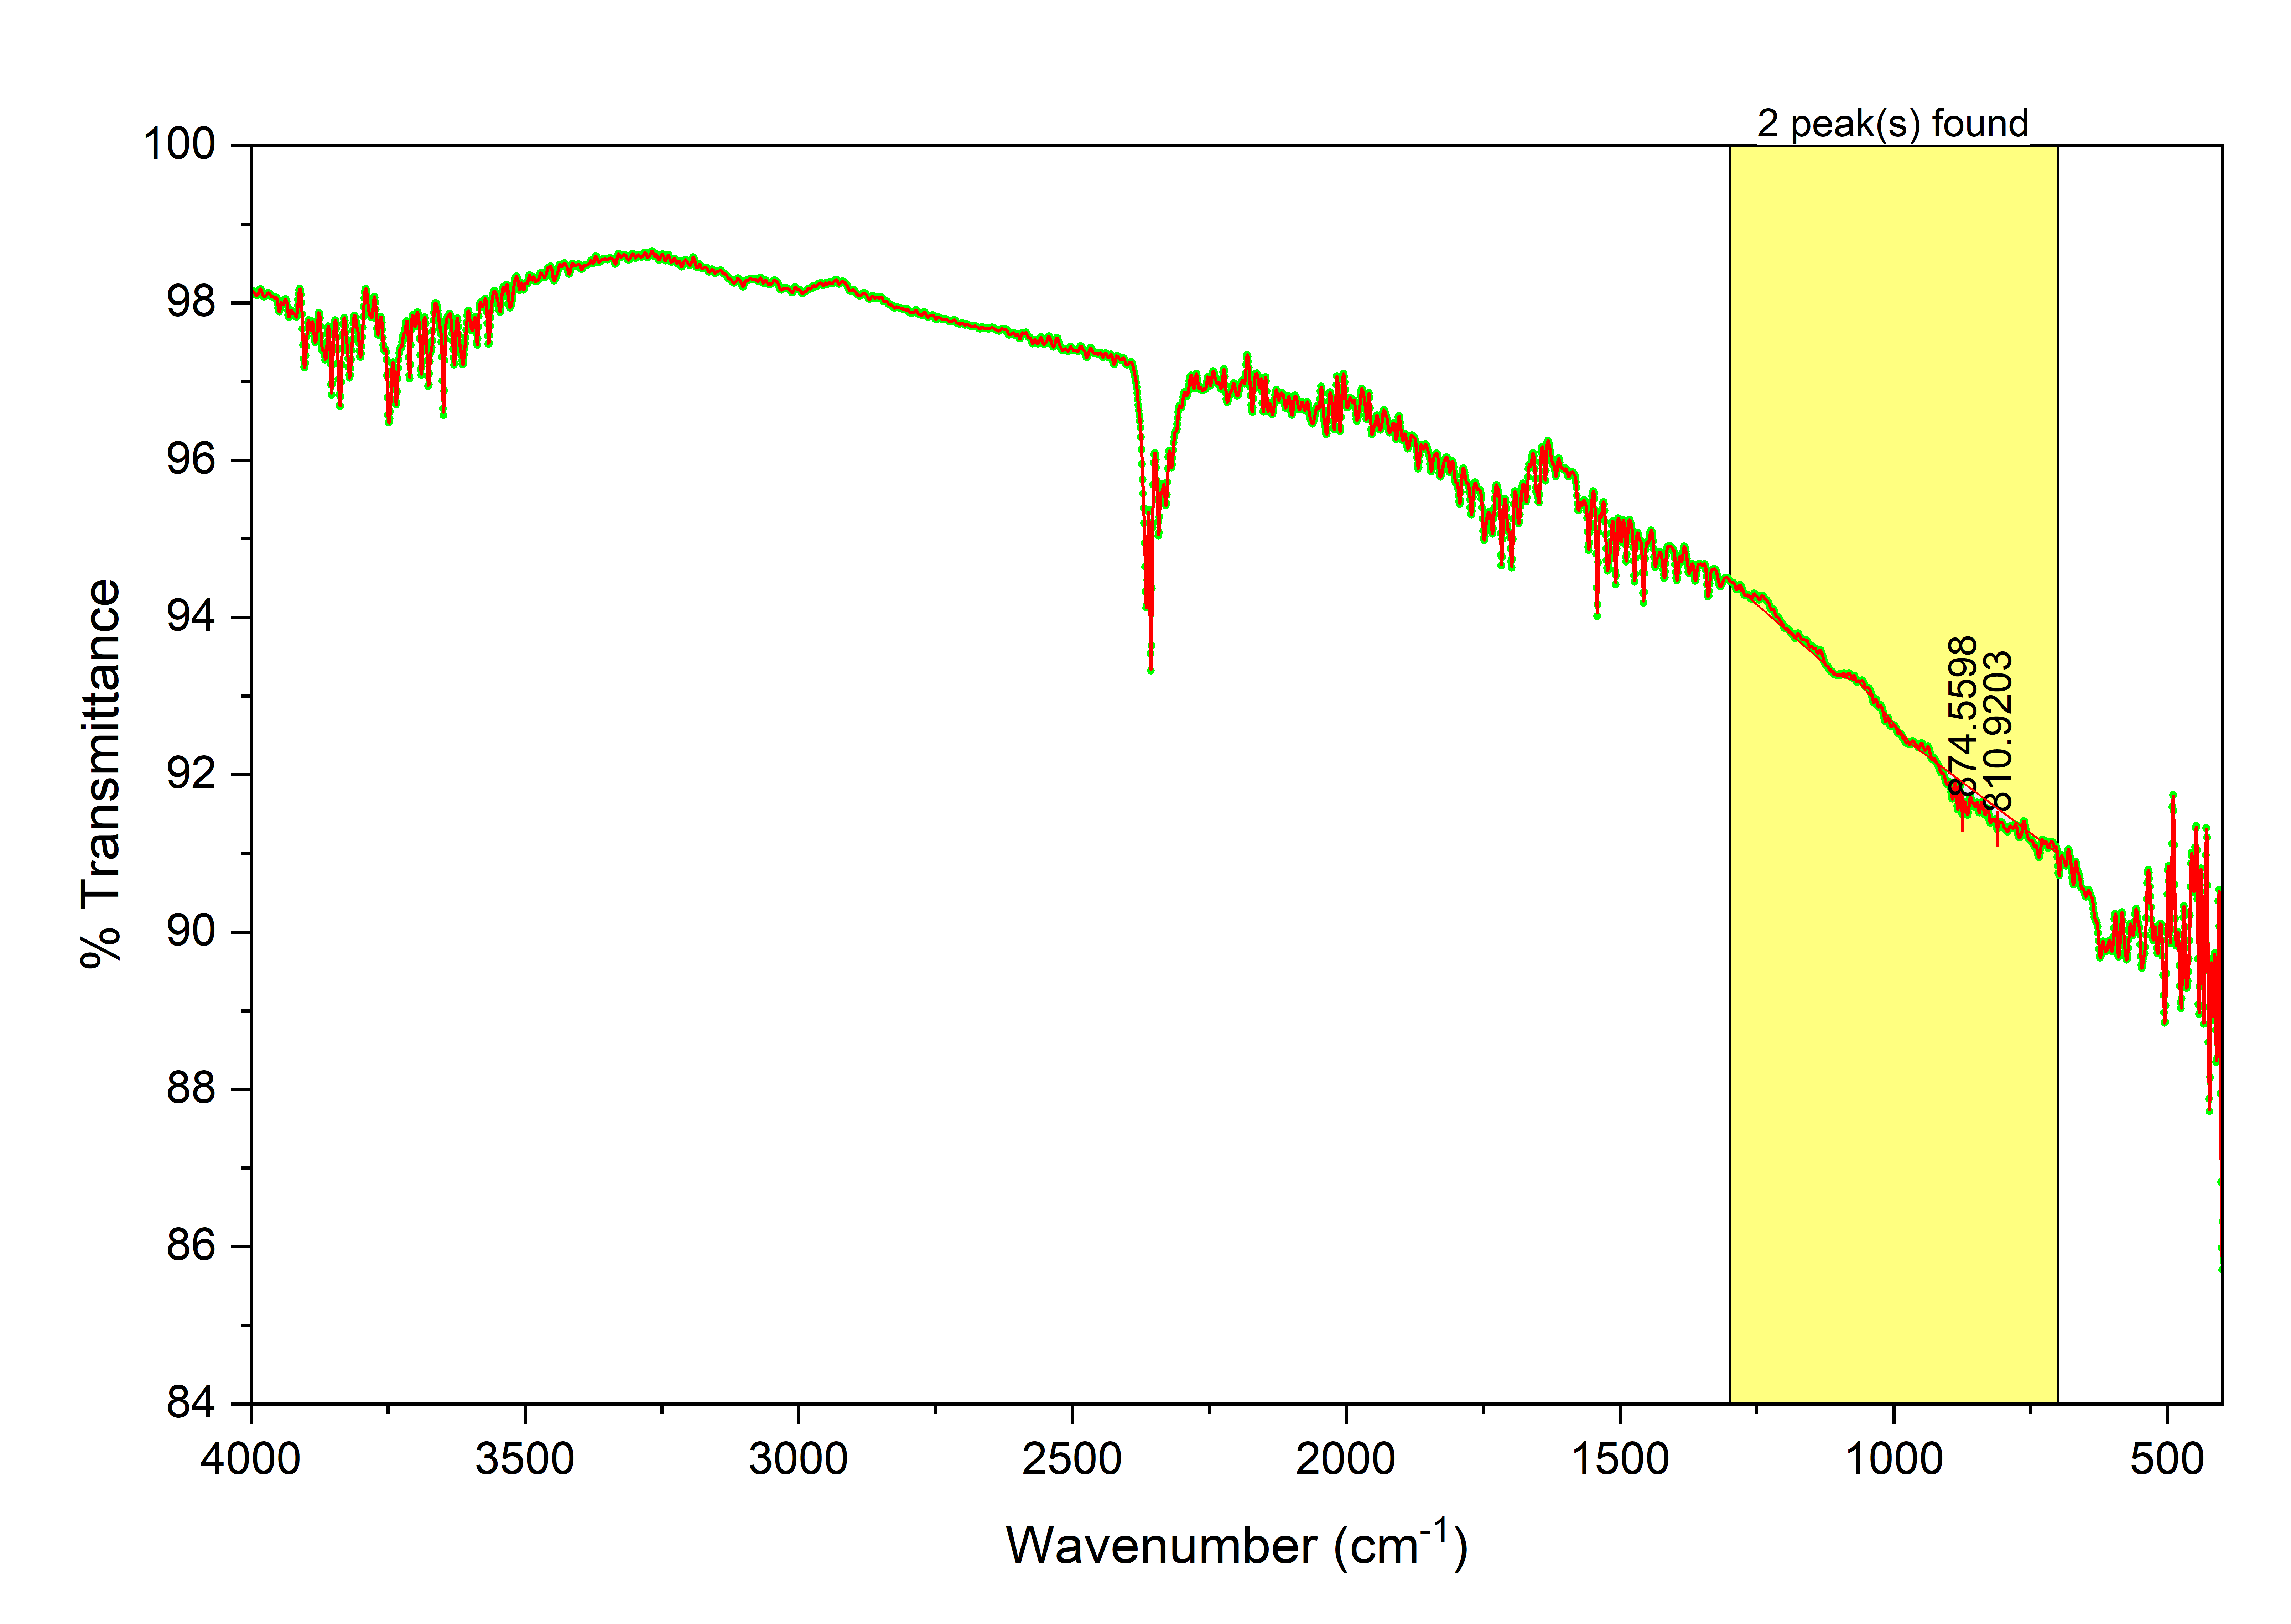
\includegraphics[width=1\textwidth]{Au-MoS2_SillicBase.png}
    \caption{Phổ FT-IR của mẫu \ce{Au-MoS2}.}
    \label{fig:ftir_aumos2}
\end{figure}
2 Peaks: 874 $cm^{-1}$, 810 $cm^{-1}$. \newline
- Nền giảm dần giống B-Ag. Au không có hấp thụ IR, còn dao động Mo-S của MoS₂ nằm ~400-480 $cm^{-1}$, đúng vùng nhiễu nên không thấy rõ. \newline
- Hai đỉnh 874 và 811 $cm^{-1}$ nằm trong vùng thường gán cho dao động Mo-O-Mo. Có thể gợi ý \ce{MoS2} bị oxi hóa một phần (\ce{MoO3}), nhưng chỉ nên viết là “có thể”, vì cường độ rất yếu.


\end{document}
